\section{Additional Estimates of Fundamental Biological Processes}
\label{sec:SI_nutr_trans}

In the main text of this work, we present estimates for a significant number of
fundamental biological processes that are necessary for cell division. While we
believe the estimates provided in the main text provide a succinct summary of
the corresponding process, we left out additional estimates of related
processes for brevity. In this section of the appendix, we present these
additional estimates in full.

\subsection{Nutrient Transport}
In the main text, we make passing mention that in typical laboratory conditions,
transport carbon often comes in the form of carbohydrates and sugar alcohols
while other critical elements -- such as nitrogen, sulfur, and phosphorus -- are
transported as inorganic ions. Below, we expand on our discussion of carbon uptake by
considering specific carbohydrate transporters and then present estimates for the transport
requirements of these other vital elements.

\subsubsection{Specific Carbon Transport}
It is important to note that so far we have neglected any specifics of the
regulation of the carbon transport system. Using the diverse array of growth
conditions available in the data, we can explore how individual carbon transport
systems depend on specific carbon availability. In
\textbf{\textit{Figure 2}}(A) of the main text, we showed the total number of
carbohydrate transporters specific to different carbon sources. A striking
observation is the  constancy in the expression of the glucose-specific
transport systems, an observation that stands in contrast with other species of
transporters [\FIG{specific_carbon_tport}(A)]. Additionally, we note that the
total number of glucose-specific transporters is tightly distributed at $\approx
1\times 10^4$ per cell, the approximate number of transporters needed to sustain
rapid growth of several divisions per hour. Interestingly, this illustrates that
\textit{E. coli} maintains a substantial number of complexes present for
transporting glucose regardless of growth condition, which is known to be the
preferential carbon source \citep{monod1947, liu2005a, aidelberg2014}.

Many metabolic operons are regulated with dual-input logic gates that are only
expressed when glucose concentrations are low and the concentration of other
carbon sources are elevated \citep{gama-castro2016, zhang2014a, gama-castro2016,
belliveau2018, ireland2020}. Points colored in red in
\FIG{specific_carbon_tport} correspond to growth conditions in which the
specific carbon source [glycerol, xylose, or fructose for (B, C, and D),
respectively] is present as the sole source of carbon. The grey lines in
\FIG{specific_carbon_tport} show the estimated number of transporters needed at
each growth rate to satisfy the cellular carbon requirement, adjusted for the
specific carbon source in terms of number of carbon atoms per molecule and the
rate of transport for the particular transporter species. These plots show that,
even in the absence of the particular carbon source, expression of the
transporters is maintained on the order of $\approx 1 \times 10^2$ per cell. The
low but non-zero abundances may reflect the specific regulatory logic involved,
requiring that cells are able to transport some minimal amount of an alternative
carbon source in order to induce expression of these alternative carbon-source
systems when needed \citep{laxhuber2020}.

\begin{figure*}
    \centering{
    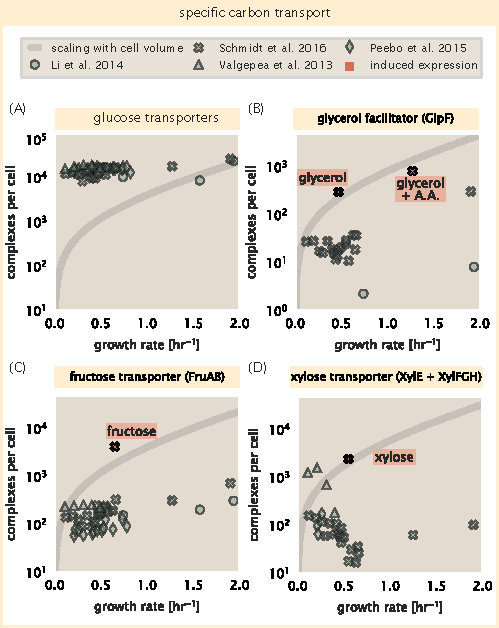
\includegraphics{SI_figs/figS1_specific_carbon.pdf}
    \caption{\textbf{The abundance of specific carbon transport systems across growth
    rates.}  Since the rates of substrate transport differ between these transporter
    species, we used the following transport rates for
    each transporter species: (A) 200
    glucose$\cdot$ s$^{-1}$ (BNID: 103693),  (B) 2000 glycerol$\cdot$s$^{-1}$
    \citep{lu2003}, (C) 200 fructose$\cdot$ s$^{-1}$ (assumed to be similar to PtsI,
    BNID: 103693), and (D) 50 xylose$\cdot$s$^{-1}$ (assumed to be comparable to
    LacY, BNID:103159). Red points and highlighted text indicate conditions in
    which the only source of carbon in the growth medium induces expression of
    the transport system. Grey lines represents the estimated
    number of transporters per cell across the continuum of growth
    rates.} \label{fig:specific_carbon_tport}
    }
\end{figure*}

\subsubsection{Nitrogen}
We must first address which elemental sources must require active transport,
meaning that the cell cannot acquire appreciable amounts simply via diffusion
across the membrane. The permeability of the lipid membrane to a large number
of solutes has been extensively characterized over the past century. Large,
polar molecular species (such as various sugar molecules, sulfate, and
phosphate) have low permeabilities while small, non-polar compounds (such as
oxygen, carbon dioxide, and ammonia) can readily diffuse across the membrane.
Ammonia, a primary source of nitrogen in typical laboratory conditions, has a
permeability on par with water ($\approx 1\times 10^{5}$ nm/s, BNID:110824). In
nitrogen-poor conditions, \textit{E. coli} expresses a transporter (AmtB)
which appears to aid in nitrogen assimilation, though the mechanism and
kinetic details of transport are still a matter of debate
\citep{heeswijk2013a, khademi2004}. Beyond ammonia, another plentiful source
of nitrogen come in the form of glutamate, which has its own complex
metabolism and scavenging pathways. However, nitrogen is plentiful in the
growth conditions examined in this work, permitting us to neglect nitrogen
transport as a potential rate limiting process in cell division in typical
experimental conditions.

\subsubsection{Phosphorus}
Phosphorus is critical to the cellular energy economy in the form of high-energy
phosphodiester bonds making up DNA, RNA, and the NTP energy pool as well as
playing a critical role in the post-translational modification of proteins and
defining the polar-heads of lipids. In total, phosphorus makes up $\approx$3\%
of the cellular dry mass which in typical experimental conditions is in the form
of inorganic phosphate. The cell membrane has remarkably low permeability to
this highly-charged and critical molecule, therefore requiring the expression of
active transport systems. In \textit{E. coli}, the proton electrochemical
gradient across the inner membrane is leveraged to transport inorganic phosphate
into the cell \citep{rosenberg1977}. Proton-solute symporters are widespread in
\textit{E. coli} \citep{ramos1977, booth1979} and can have rapid transport rates
of 50 to 100 molecules per second for sugars and other solutes (BNID: 103159;
111777). As a more extreme example, the proton transporters in the F$_1$-F$_0$
ATP synthase, which use the proton electrochemical gradient for rotational
motion, can shuttle protons across the membrane at a rate of $\approx$ 1000 per
second (BNID: 104890; 103390).

In \textit{E. coli} the PitA phosphate transport system has been shown to be
very tightly coupled with the proton electrochemical gradient with a 1:1
proton:phosphate stoichiometric ratio \citep{harris2001, feist2007}. Taking the
geometric mean of the aforementioned estimates gives a plausible rate of
phosphate transport on the order of 300  per second. Illustrated in
\textbf{\textit{Figure 2}}(B), we can estimate that $\approx$ 200 phosphate
transporters are necessary to maintain an $\approx$ 3\% dry mass with a 5000 s
division time. This estimate is consistent with observation when we examine the
observed copy numbers of PitA in proteomic data sets (plot in
\textbf{\textit{Figure 2}}(B)). While our estimate is very much in line with the
observed numbers, we emphasize that this is likely a slight overestimate of the
number of transporters needed as there are other phosphorous scavenging systems,
such as the ATP-dependent phosphate transporter Pst system which we have
neglected.

\subsubsection{Sulfur}
Similar to phosphate, sulfate is highly-charged and not particularly membrane
permeable, requiring active transport. While there exists a H+/sulfate
symporter in \textit{E. coli}, it is in relatively low abundance and is not
well characterized \citep{zhang2014}. Sulfate is predominantly acquired via
the ATP-dependent ABC transporter CysUWA system which also plays an important
role in selenium transport \citep{sekowska2000, sirko1995}. While specific
kinetic details of this transport system are not readily available, generic
ATP transport systems in prokaryotes transport on the order of 1 to 10
molecules per second (BNID: 109035). Combining this generic transport rate,
measurement of sulfur comprising 1\% of dry mass, and a 5000 second division
time yields an estimate of $\approx$ 1000 CysUWA complexes per cell
[\textbf{\textit{Figure 2}}(C)]. Once again, this estimate is in notable
agreement with proteomic data sets, suggesting that there are sufficient
transporters present to acquire the necessary sulfur. In a similar spirit of
our estimate of phosphorus transport, we emphasize that this is likely an
overestimate of the number of necessary transporters as we have neglected
other sulfur scavenging systems that are in lower abundance.



\subsection{Additional Process of the Central Dogma}
\label{sec:SI_central_dogma}
In the main text, we consider the processes underlying the backbone of the
central dogma, namely DNA replication, RNA transcription, and protein
translation. In this section we expand on our discussion of DNA replication and also
turn our attention to additional processes
related to the central dogma, primarily dNTP synthesis for DNA replication and
amino-acyl tRNA synthesis for translation. Additionally, we explore in more
detail the estimates shown in \textbf{\textit{Figure 4}}(A) for the RNA polymerase
requirements of mRNA and tRNA synthesis.

\subsection{DNA Replication}
To successfully divide and produce viable progeny, the DNA must be
faithfully replicated and segregated into each nascent cell. Most bacteria
(including \textit{E. coli}) harbor a single, circular chromosome and can have
extra-chromosomal plasmids up to $\sim$ 100 kbp in length. Replication is initiated at a single region of the
chromosome termed the \textit{oriC} locus where a pair of replisomes, each
consisting of two DNA polymerase III, begin their high-fidelity replication of
the genome in opposite directions \citep{fijalkowska2012}. \textit{In vitro}
measurements have shown that DNA Polymerase III copies DNA at a rate of $\approx
600$ nucleotides per second (BNID: 104120). To replicate a single chromosome of
$\approx 5\times 10^6$ base pairs, two replisomes moving at their maximal rate
would copy the entire genome in $\approx$ 4000 s; well within our division time
of 5000 seconds.

In rapidly growing cultures, bacteria like \textit{E. coli} can initiate as many
as 10 - 12 replication forks at a given time \citep{bremer2008, si2017},
suggesting  only $\approx 10$ are needed. However, as shown in
\textbf{\textit{Figure 4}}(A), DNA polymerase III is nearly an order of magnitude more
abundant but still maintains the expected growth rate dependence. This
discrepancy can be understood by considering its binding constant to DNA as we noted in
the main text and plotted in  \textbf{\textit{Figure 4}}(B).
The concentration of DNA polymerase III across
all data sets apear in this range and cells vary their copy number such that its
concentration is approximately equal to the dissociation constant to the DNA.
While the processes regulating the initiation of DNA replication are complex and
involve more than just the holoenzyme, these data indicate that the kinetics of
replication rather than the explicit copy number of the DNA polymerase III
holoenzyme is the more relevant feature of DNA replication to consider. In light
of this, DNA replication does not represent a rate-limiting step in
cell division. Interestingly, it is worth noting that for bacterium like \textit{C.
crescentus} whose chromosomal replication is initiated only once per cell cycle
\citep{jensen2001}, the time to double their chromosome indeed represents an
upper limit to their growth rate.

\subsubsection{dNTP synthesis}
The four major dNTPs (dATP, dTTP, dCTP, and dGTP) serve as the fundamental
units of the genetic code. Thus, to faithfully replicate the chromosome, the
cell must be able to synthesize enough of these bases in the first place. All
dNTPs are synthesized \textit{de novo} in separate pathways, requiring
different building blocks. However, a critical step present in all dNTP
synthesis pathways is the conversion from ribonucleotide to
deoxyribonucleotide via the removal of the 3' hydroxyl group of the ribose
ring \citep{rudd2016}. This reaction is mediated by a class of enzymes termed
ribonucleotide reductases, of which \textit{E. coli} possesses two
aerobically active complexes (termed I and II) and a single anaerobically
active enzyme. Due to their peculiar formation of a radical intermediate,
these enzymes have received much biochemical, kinetic, and structural
characterization. One such work \citep{ge2003} performed a detailed
\textit{in vitro} measurement of the steady-state kinetic rates of these
complexes, revealing a turnover rate of $\approx$ 10 dNTP per second.

Since this reaction is central to the synthesis of all dNTPs, it is reasonable
to consider the abundance of these complexes is a measure of the total dNTP
production in \textit{E. coli}. We consider the fact that to replicate the
cell's genome, on the order of $\approx 1\times 10^{7}$ dNTPs must be
synthesized. Assuming a production rate of 10 per second per ribonucleotide
reductase complex and a cell division time of 5000 seconds, we arrive at an
estimate of $\approx$ 200 complexes needed per cell. We find that this estimate
agrees with the experimental measurements of these complexes abundances within
$\approx 1/2$ an order of magnitude. Extension of this estimate across a
continuum of growth rate, including the fact that multiple chromosomes can be
replicated at a given time, is shown as a grey transparent line in
\textbf{\textit{Figure 7–Figure Supplement 1}}.  Similarly to our point
estimate, we find that this estimate agrees  across a continuum of growth rate,
including the fact that multiple chromosomes can be replicated at a given time.

Recent work has revealed that during replication, the ribonucleotide
reductase complexes coalesce to form discrete foci colocalized with the DNA
replisome complex \citep{sanchez-romero2011}. This is particularly pronounced
in conditions where growth is slow, indicating that spatial organization and
regulation of the activity of the complexes plays an important role.

\subsubsection{mRNA and tRNA Synthesis}
Here we expand on our discussion on RNA polymerase and consider the synthesis of
mRNA and tRNA. In \textbf{\textit{Figure 4}}(B,C) of the main text, we plotted
the measured  number of core RNA polymerase, as well as the number of RpoD sigma
factors.

To form a functional protein, all protein coding genes must first be
transcribed from DNA to form a mRNA molecule. While each protein requires an
mRNA blueprint, many copies of the protein can be synthesized from a single
mRNA. Factors such as strength of the ribosomal binding site, mRNA stability,
and rare codon usage frequency dictate the number of proteins that can be
made from a single mRNA, with yields ranging from 10$^1$ to 10$^4$ (BNID:
104186; 100196; 106254). Computing the geometric mean of this range yields
$\approx$ 1000 proteins synthesized per mRNA, a value that agrees with
experimental measurements of the number of proteins per cell ($\approx 3
\times 10^6$, BNID: 100088) and total number of mRNA per cell ($\approx 3
\times 10^3$, BNID:100064).

This estimation captures the \textit{steady-state} mRNA copy number, meaning
that at any given time, there will exist approximately 3000 unique mRNA
molecules. To determine the \textit{total} number of mRNA that need to be
synthesized over the cell's lifetime, we must consider degradation of the
mRNA. In most bacteria, mRNAs are rather unstable with life times on the
order of several minutes (BNID: 104324; 106253; 111927; 111998). For
convenience, we assume that the typical mRNA in our cell of interest has a
typical lifetime of $\approx$ 300 seconds. Using this value, we can determine
the total mRNA production rate to maintain a steady-state copy number of 3000
mRNA per cell. While we direct the reader to the appendix for a more detailed
discussion of mRNA transcriptional dynamics, we state here that the total
mRNA production rate must be on the order of $\approx$ 15 mRNA per second. In
\textit{E. coli}, the average protein is $\approx$ 300 amino acids in length
(BNID: 108986), meaning that the corresponding mRNA is $\approx$ 900
nucleotides which we will further approximate as $\approx$ 1000 nucleotides
to account for the non-protein coding regions on the 5' and 3' ends. This
means that the cell must have enough RNA polymerase molecules around to
sustain a transcription rate of $\approx 1.5 \times 10^4$ nucleotides per
second. Knowing that a single RNA polymerase polymerizes RNA at a clip of 40
nucleotides per second, we arrive at a comfortable estimate of $\approx$ 250
RNA polymerase complexes needed to satisfy the mRNA demands of the cell. It
is worth noting that this number is approximately half of that required to
synthesize enough rRNA, as we saw in the previous section. We find this to be
a striking result as these 250 RNA polymerase molecules are responsible for
the transcription of the $\approx$ 4000 protein coding genes that are not
ribosome associated.

We now turn our attention to the synthesis of tRNA. Unlike mRNA or rRNA, each
individual tRNA is remarkably short, ranging from 70 to 95 nucleotides each
(BNID: 109645; 102340). What they lack in length, they make up for in
abundance, with reported values ranging from $\approx$ 5 $\times$10$^4$ (BNID:
105280) to $\approx$ 5 $\times$10$^5$ (BNID: 108611). To test tRNA synthesis as
a possible growth-rate limiting stage, we will err towards a higher abundance
of $\approx$ 5$\times$10$^5$ per cell. Combining the abundance and tRNA
length measurements, we make the estimate that $\approx 5 \times 10^7$
nucleotides are sequestered in tRNA per cell. Unlike mRNA, tRNA is remarkably
stable with typical lifetimes \textit{in vivo} on the order of $\approx$ 48
hours \citep{abelson1974,svenningsen2017} -- well beyond the timescale of
division. Once again using our rule-of-thumb for the rate of transcription to
be 40 nucleotides per second and assuming a division time of $\approx$ 5000
seconds, we arrive at an estimate of $\approx$ 200 RNA polymerases to
synthesize enough tRNA. This requirement pales in comparison to the number of
polymerases needed to generate the rRNA and mRNA pools and can be neglected
as a significant transcriptional burden.

\subsubsection{tRNA Charging}
In the previous subsection, we focused solely on estimating the number of RNA
polymerases needed for the generation of the tRNA molecule itself. We now
explore the protein complex requirements for ligation of the appropriate
amino acid to each tRNA. We begin by again using an estimate of $\approx$
$\approx 3\times 10^{6}$ proteins per cell at a 5000 s division time (BNID: 115702)
and a typical protein length of $\approx$ 300 amino acids (BNID: 100017), we
can estimate that a total of $\approx 1\times 10^{9}$ amino acids are stitched
together by peptide bonds.

How many tRNAs are needed to facilitate this remarkable number of amino acid
delivery events to the translating ribosomes? It is important to note that
tRNAs are recycled after they've passed through the ribosome and can be
recharged with a new amino acid, ready for another round of peptide bond
formation. While some \textit{in vitro} data exists on the turnover of tRNA
in \textit{E. coli} for different amino acids, we can make a reasonable
estimate by comparing the number of amino acids to be polymerized to cell
division time. Using our stopwatch of 5000 s and $\approx 1\times 10^{9}$ amino acids, we
arrive at a requirement of $\approx 2\times 10^{5}$ tRNA molecules to be
consumed by the ribosome per second.

There are many processes which go into synthesizing a tRNA and ligating it
with the appropriate amino acids. As we discussed previously, there appear to
be more than enough RNA polymerases per cell to synthesize the needed pool of
tRNAs. Without considering the many ways in which amino acids can be
scavenged or synthesized \textit{de novo}, we can explore ligation the as a
potential rate limiting step. The enzymes which link the correct amino acid
to the tRNA, known as tRNA synthetases or tRNA ligases, are incredible in
their proofreading of substrates with the incorrect amino acid being ligated
once out of every $10^4$ to $10^5$ events (BNID: 103469). This is due in part
to the consumption of energy as well as a multi-step pathway to ligation.
While the rate at which tRNA is ligated is highly dependent on the identity
of the amino acid, it is reasonable to state that the typical tRNA synthetase
has charging rate of $\approx$ 20 AA per tRNA synthetase per second (BNID:
105279).

We can make an assumption that amino-acyl tRNAs are in steady-state where
they are produced at the same rate they are consumed, meaning that $2 \times
10^5$ tRNAs must be charged per second. Combining these estimates together,
as shown schematically in \textbf{\textit{Figure 4}}(F), yields an estimate of $\approx 1\times 10^{4}$
tRNA synthetases per cell with a division time of 5000 s. This point estimate
is in very close agreement with the observed number of synthetases (the sum
of all 20 tRNA synthetases in \textit{E. coli}). This estimation strategy
seems to adequately describe the observed growth rate dependence of the tRNA
synthetase copy number (shown as the grey line in \textbf{\textit{Figure 4}}(F), suggesting
that the copy number scales with the cell volume.

In total, the estimated and observed $\approx 1\times 10^{4}$ tRNA synthetases occupy
only a meager fraction of the total cell proteome, around 0.5\% by abundance.
It is reasonable to assume that if tRNA charging was a rate limiting process,
cells would be able to increase their growth rate by devoting more cellular
resources to making more tRNA synthases. As the synthesis of tRNAs and the
corresponding charging can be highly parallelized, we can argue that tRNA
charging is not a rate limiting step in cell division, at least for the
growth conditions explored in this work.
